\section{Methods for concept drift adaptation}
% ------------------------------------------------------------------------------
\begin{frame}
\frametitle{Agenda}
\tableofcontents[currentsection]
\end{frame}
% ------------------------------------------------------------------------------


% --------------------------------------------------------------------------------------------------------------
\begin{frame}
\frametitle{Methods for concept drift Adaptation}

\begin{figure}[H]
	\centering
	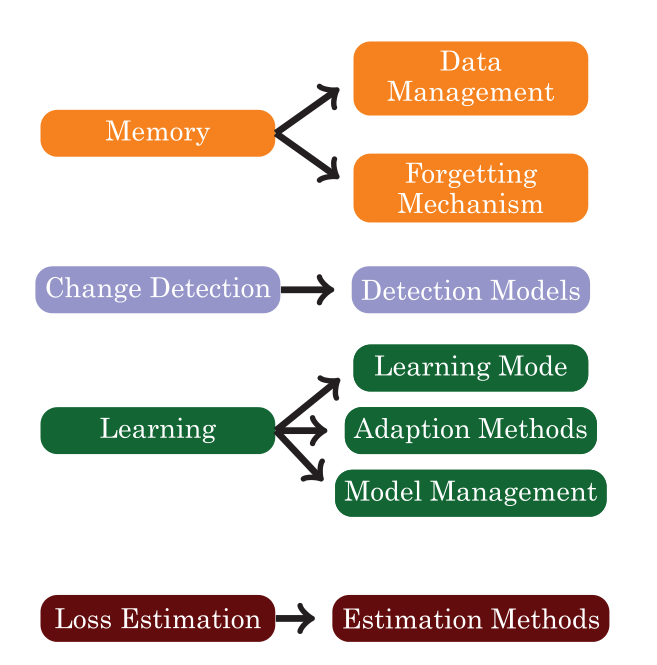
\includegraphics[scale=0.25]{mfcda/fourmodules}
\end{figure}

\end{frame}
% --------------------------------------------------------------------------------------------------------------

\subsection{Memory}

% ------------------------------------------------------------------------------
\begin{frame}
\frametitle{Agenda}
\tableofcontents[currentsubsection]
\end{frame}
% ------------------------------------------------------------------------------

% --------------------------------------------------------------------------------------------------------------
\begin{frame}
\frametitle{Memory in concept drift Adaptation}

\begin{figure}[H]
	\centering
	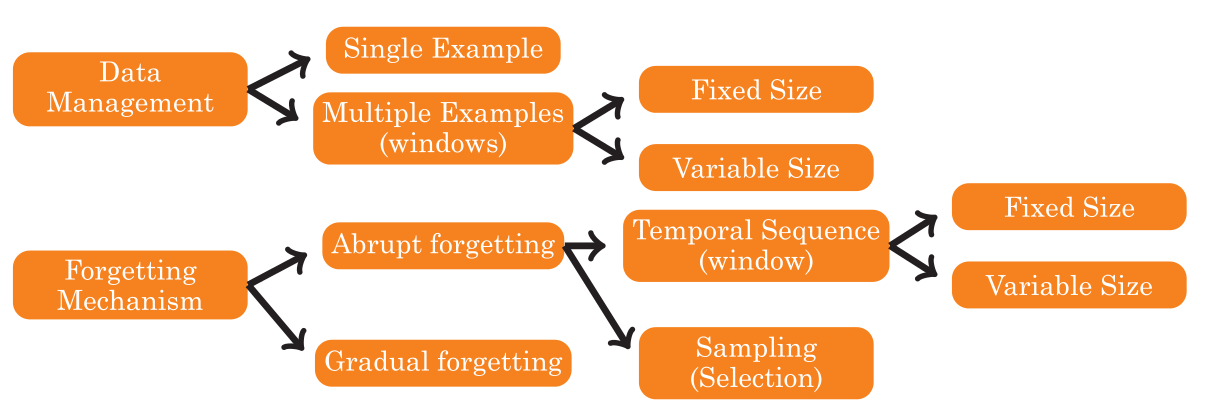
\includegraphics[width=\textwidth]{mfcda/memory}
\end{figure}

\end{frame}
% --------------------------------------------------------------------------------------------------------------








\subsection{Change Detection}

% ------------------------------------------------------------------------------
\begin{frame}
\frametitle{Agenda}
\tableofcontents[currentsubsection]
\end{frame}
% ------------------------------------------------------------------------------



\subsection{Learning}

% ------------------------------------------------------------------------------
\begin{frame}
\frametitle{Agenda}
\tableofcontents[currentsubsection]
\end{frame}
% ------------------------------------------------------------------------------

\begin{frame}



\end{frame}







\subsection{Loss Estimation}

% ------------------------------------------------------------------------------
\begin{frame}
\frametitle{Agenda}
\tableofcontents[currentsubsection]
\end{frame}
% ------------------------------------------------------------------------------


% --------------------------------------------------------------------------------------------------------------
\begin{frame}
\frametitle{Loss estimation in concept drift Adaptation}

\begin{figure}[H]
	\centering
	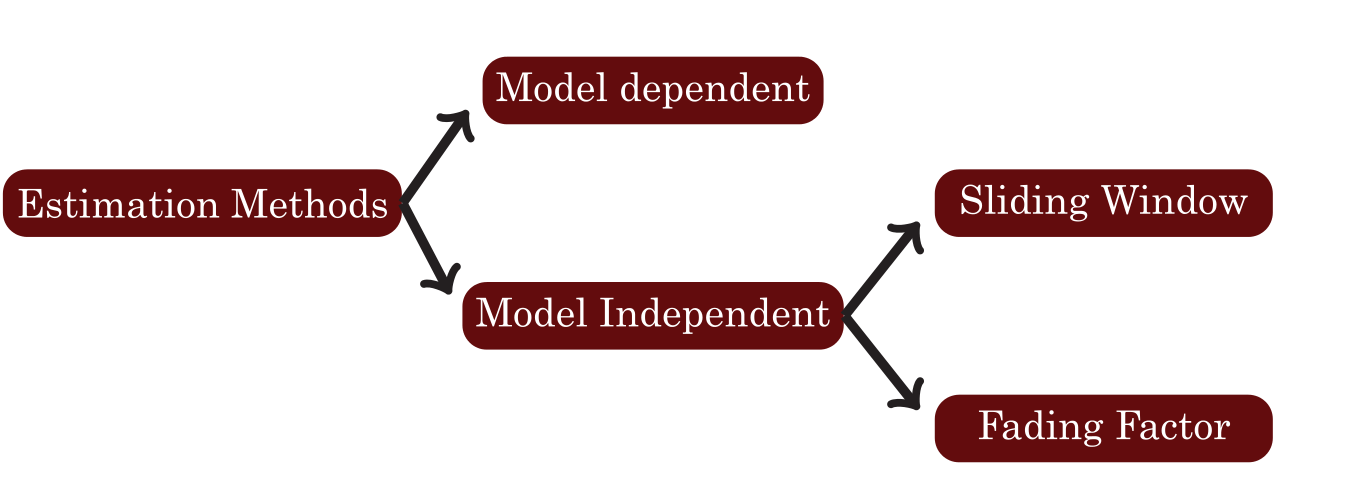
\includegraphics[scale=0.2]{mfcda/loss}
\end{figure}
\only<2>{
\begin{itemize}

\item \textbf{Model Dependent}
	\begin{itemize}
	\item Estimator needs to learn from the current model
	\item e.g. Klinkenbeg and Joachims \cite{klinkenberg} use it in SVM
	\end{itemize}

\end{itemize}
}

\only<3>{
\begin{itemize}

\item \textbf{Model Independent}
	\begin{itemize}
	\item Can be applied immediately
	\item \textbf{Sliding Window:} one small (quick) and one large (slower) together
	\item \textbf{Fading Factor:} a small FF detects change earlier
	\end{itemize}
\end{itemize}
}

\end{frame}




% --------------------------------------------------------------------------------------------------------------
